% So we make this "beamer" rather than document!

\documentclass[11pt]{beamer}
% For handout add ,handout after 11pt

\usetheme[sectionpage=none,numbering=none]{metropolis}           % Use metropolis theme
	% To do printouts, add ", handout"  after aspectratio.
\usepackage{booktabs}
\usepackage{graphicx}
\usepackage{color}

\title{Machine Learning Bias}
\author{\small Nick Eubank}
\date{\vspace*{.3in} \date}


% This is the beginning of a real document!
\begin{document}


\begin{frame}
\maketitle
\end{frame}

\begin{frame}[c]{Outline}
  \begin{enumerate}
    \item How Bias Sneaks In (Biased Factors)
    \pause \item How Bias Sneaks In (Biased Measures)
    \pause \item Ethics of Type 1 versus Type 2 Errors
    \pause \item Right to Review and Black Box Algorithms
  \end{enumerate}
\end{frame}

\begin{frame}[c]{Supervised Machine Learning}
  Conceptual that because Supervised Machine Learning (SML) is built on math, it can't be biased. \\
  \pause
  \vspace{0.2cm}
  When bias creeps in, it is assumed to be because of researcher negligence. \\
  \vspace{0.2cm}
  \pause \emph{By design,} SML will always try and be biased.
\end{frame}

\begin{frame}[c]{Supervised Machine Learning}
  SML models are designed to find any patterns they can to help predict outcomes / classify records. \\
  \vspace{0.2cm}
  Because sexism, racism, xenophobia, homophobia, etc. shape outcomes in the world, \\
  \vspace{0.2cm}
  $\leadsto$ SMLs generally \alert{perform better} when they are sexist/racist/xenophobic/homophobic!
\end{frame}

\begin{frame}[c]{Supervised Machine Learning}
  We're building SML model designed to predict performance reviews using resumes.\\
  \pause Train using resumes and performance evaluations of current employees.
  \begin{itemize}
    \pause \item Help decide who to hire.
  \end{itemize}
  \pause
  \vspace{0.1cm}
  If supervisors tend to discriminate against women, then our SML will \alert{look for signals that an applicant is a woman}, since they can use this to give women lower reviews, better matching the training data.
\end{frame}

\begin{frame}[c]{Proxies}
  OK, but what if I don't include data on gender, race, sexuality, etc. in my model? \\
  \vspace{0.1cm}
  \emph{Everything} in society is correlated:
  \begin{itemize}
    \pause \item Going to a women's college (Scripps College, Barnard College)
    \pause \item Going to a Historical Black University (Howard University)
    \pause \item Many activities are gender-correlated (Yoga, Football)
    \pause \item Geography is \emph{extremely} correlated with race and income (Princeton Review)
  \end{itemize}
  \pause In COMPAS, \alert{race wasn't in the model}.
\end{frame}

\begin{frame}[c]{Biased By Design}
  Bias in Machine Learning isn't the result of negligence. \\
\vspace{0.3cm}
  \pause \alert{So long as society has biases}, Machine Learning has an \alert{affirmative incentive} to be biased too!
\end{frame}

\begin{frame}[c]{What Can I Do To Prevent Bias?}
\textbf{1. Target an unbiased outcome.}
\begin{itemize}
  \pause \item In hiring example, variables correlated with gender created bias because the target (performance evaluations) were biased!
\end{itemize}
\pause Less biased targets will reduce the incentive for your algorithm to be biased. \\
\pause Picking unbiased outcomes is not as easy as it seems...
\end{frame}

\begin{frame}[c]{What Can I Do To Prevent Bias?}
  COMPAS: Predicted probability of future arrest. \\
  \pause Arrests are pretty objective, right?
\end{frame}

\begin{frame}[c]{}
  \begin{figure}
    \centering
    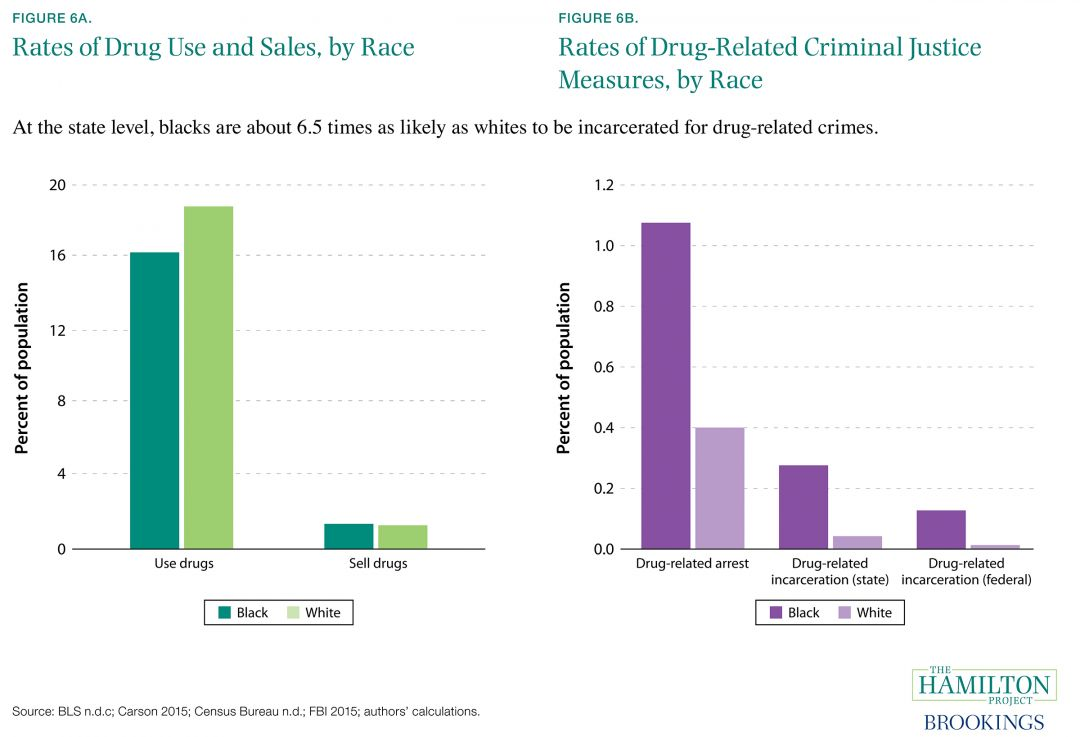
\includegraphics[width=\textwidth]{images/drug_use_versus_arrest.jpg}
  \end{figure}
  Probability of arrest $\neq$ probability of committing a crime
\end{frame}

\begin{frame}[c]{What Can I Do To Prevent Bias?}
\textbf{2. Test your models \emph{thoroughly.}} \\
COMPAS:
\begin{itemize}
  \item Same accuracy scores for Black and White suspects!
  \pause \item But... very different rates of false positives and false negatives.
\end{itemize}
\end{frame}

\begin{frame}[c]{What Can I Do To Prevent Bias?}
\textbf{3. Try to Use Interpretable Models}
\begin{figure}
  \centering
\pause 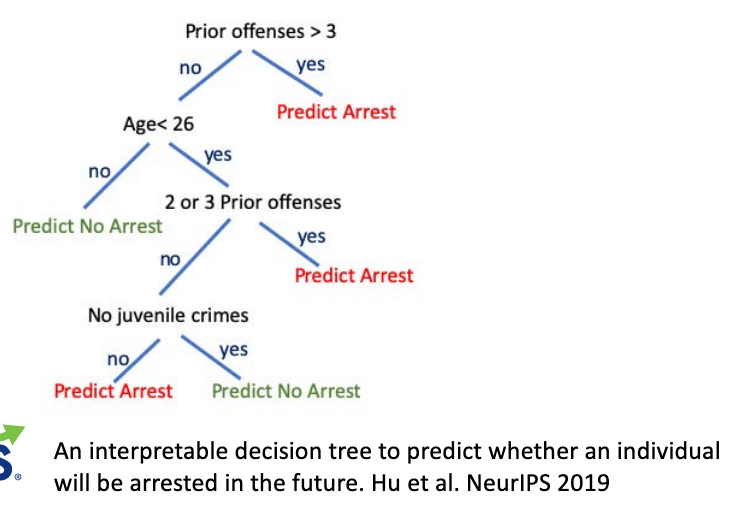
\includegraphics[width=\textwidth]{images/rudin_model_compas.png}
\end{figure}
\pause Don't preclude bias, but make models easier to audit!
\end{frame}


\end{document}
